\documentclass[conference]{IEEEtran}

\usepackage{array}
\usepackage{booktabs}
\usepackage{graphicx}
\usepackage{url}

\graphicspath{{../final-presentation/assets/}}

\begin{document}

\title{Rover Ready: A WebXR Rover Repair Bay}

\author{
	\IEEEauthorblockN{Chirag Baviskar \qquad Dhrumil Patel}
	\IEEEauthorblockA{Rutgers University\\
		Virtual Reality \& Lab, Project 2}
}

\maketitle

\begin{abstract}
	Rover Ready is a browser-based WebXR repair experience built around a compact
	low-poly rover service bay. The player calls a rover into the garage, installs
	power cells, repairs highlighted components with a handheld tool, replaces
	missing parts, checks the rover, and sends it back out. The project combines
	custom Blender-made assets, Three.js rendering, WebXR input, GLTF model loading,
	and Cannon-ES physics to create a focused interaction loop that is more complete
	than a static scene or a lightly reskinned lab exercise.
\end{abstract}

\begin{IEEEkeywords}
	WebXR, Three.js, Blender, Cannon-ES, GLTFLoader, virtual reality
\end{IEEEkeywords}

\section{Project Overview}

Rover Ready is an interactive VR scene for Rutgers Virtual Reality \& Lab
Project 2. The experience places the user inside one industrial garage bay on a
Mars service site. Instead of building a large map, the project focuses on one
room and one repeated job: prepare a rover so it can leave the bay.

The final demo is built with Three.js and WebXR, with runtime models loaded as
separate GLB files through GLTFLoader. Cannon-ES is used for physical behavior
on loose tools, power cells, and rover parts. The main visible models were
created for this project in Blender: the garage bay, the regular service rover,
the larger complex rover, the power cell, and the handheld repair tool.

The advanced features implemented for the project are physics and multiple
object types or modes. Physics gives grabbable objects weight and lets loose
parts rest on the work surfaces. Multiple object behavior appears through bay
buttons, power cells, repair targets, missing parts, regular and complex rovers,
and the repair tool. The Blender Python scripts also support the project by
procedurally generating and exporting the custom models.

\section{Scene and Interaction Description}

The scene is a single low-poly garage bay with a tool table on one side, a
diagnostic screen at the back, a bay door at the front, and a button panel for
calling, checking, and launching rovers. A Mars exterior model sits beyond the
door so the garage feels connected to a larger setting without requiring player
navigation through another area. The player can move with desktop fallback
controls or with WebXR controller thumbsticks.

The core loop begins when the player presses the call button. The bay door opens
and a rover arrives at the marked work zone. On early levels, the player grabs a
power cell from the rack and moves it into the receiver on the rover. The power
cell remains a loose physics object until it is close enough to the named snap
target on the rover. At that point, it snaps into the dock, locks in place, and
updates the rover state.

The repair interaction uses a separate handheld tool. The player grabs the tool
and aims its tip at damaged rover components. Damaged targets glow while the tool
is aimed correctly, and holding the tool on the target long enough marks the
component as repaired. Later levels add missing-part tasks. Parts such as panels,
wheels, lights, bumpers, and science pods spawn as loose grabbable objects on
the tool table, and the player must place them near their matching rover snap
targets before the check sequence succeeds.

Progression keeps the same readable loop while increasing the amount of work. A
regular rover is used for the first levels. At level six and beyond, the demo
switches to a larger complex rover with two power-cell slots and more possible
repair and replacement targets.

\noindent\textbf{Demo video link:} \textit{Add the final uploaded 1--2 minute
	demo video URL here before submission.}

\begin{figure*}[t]
	\centering
	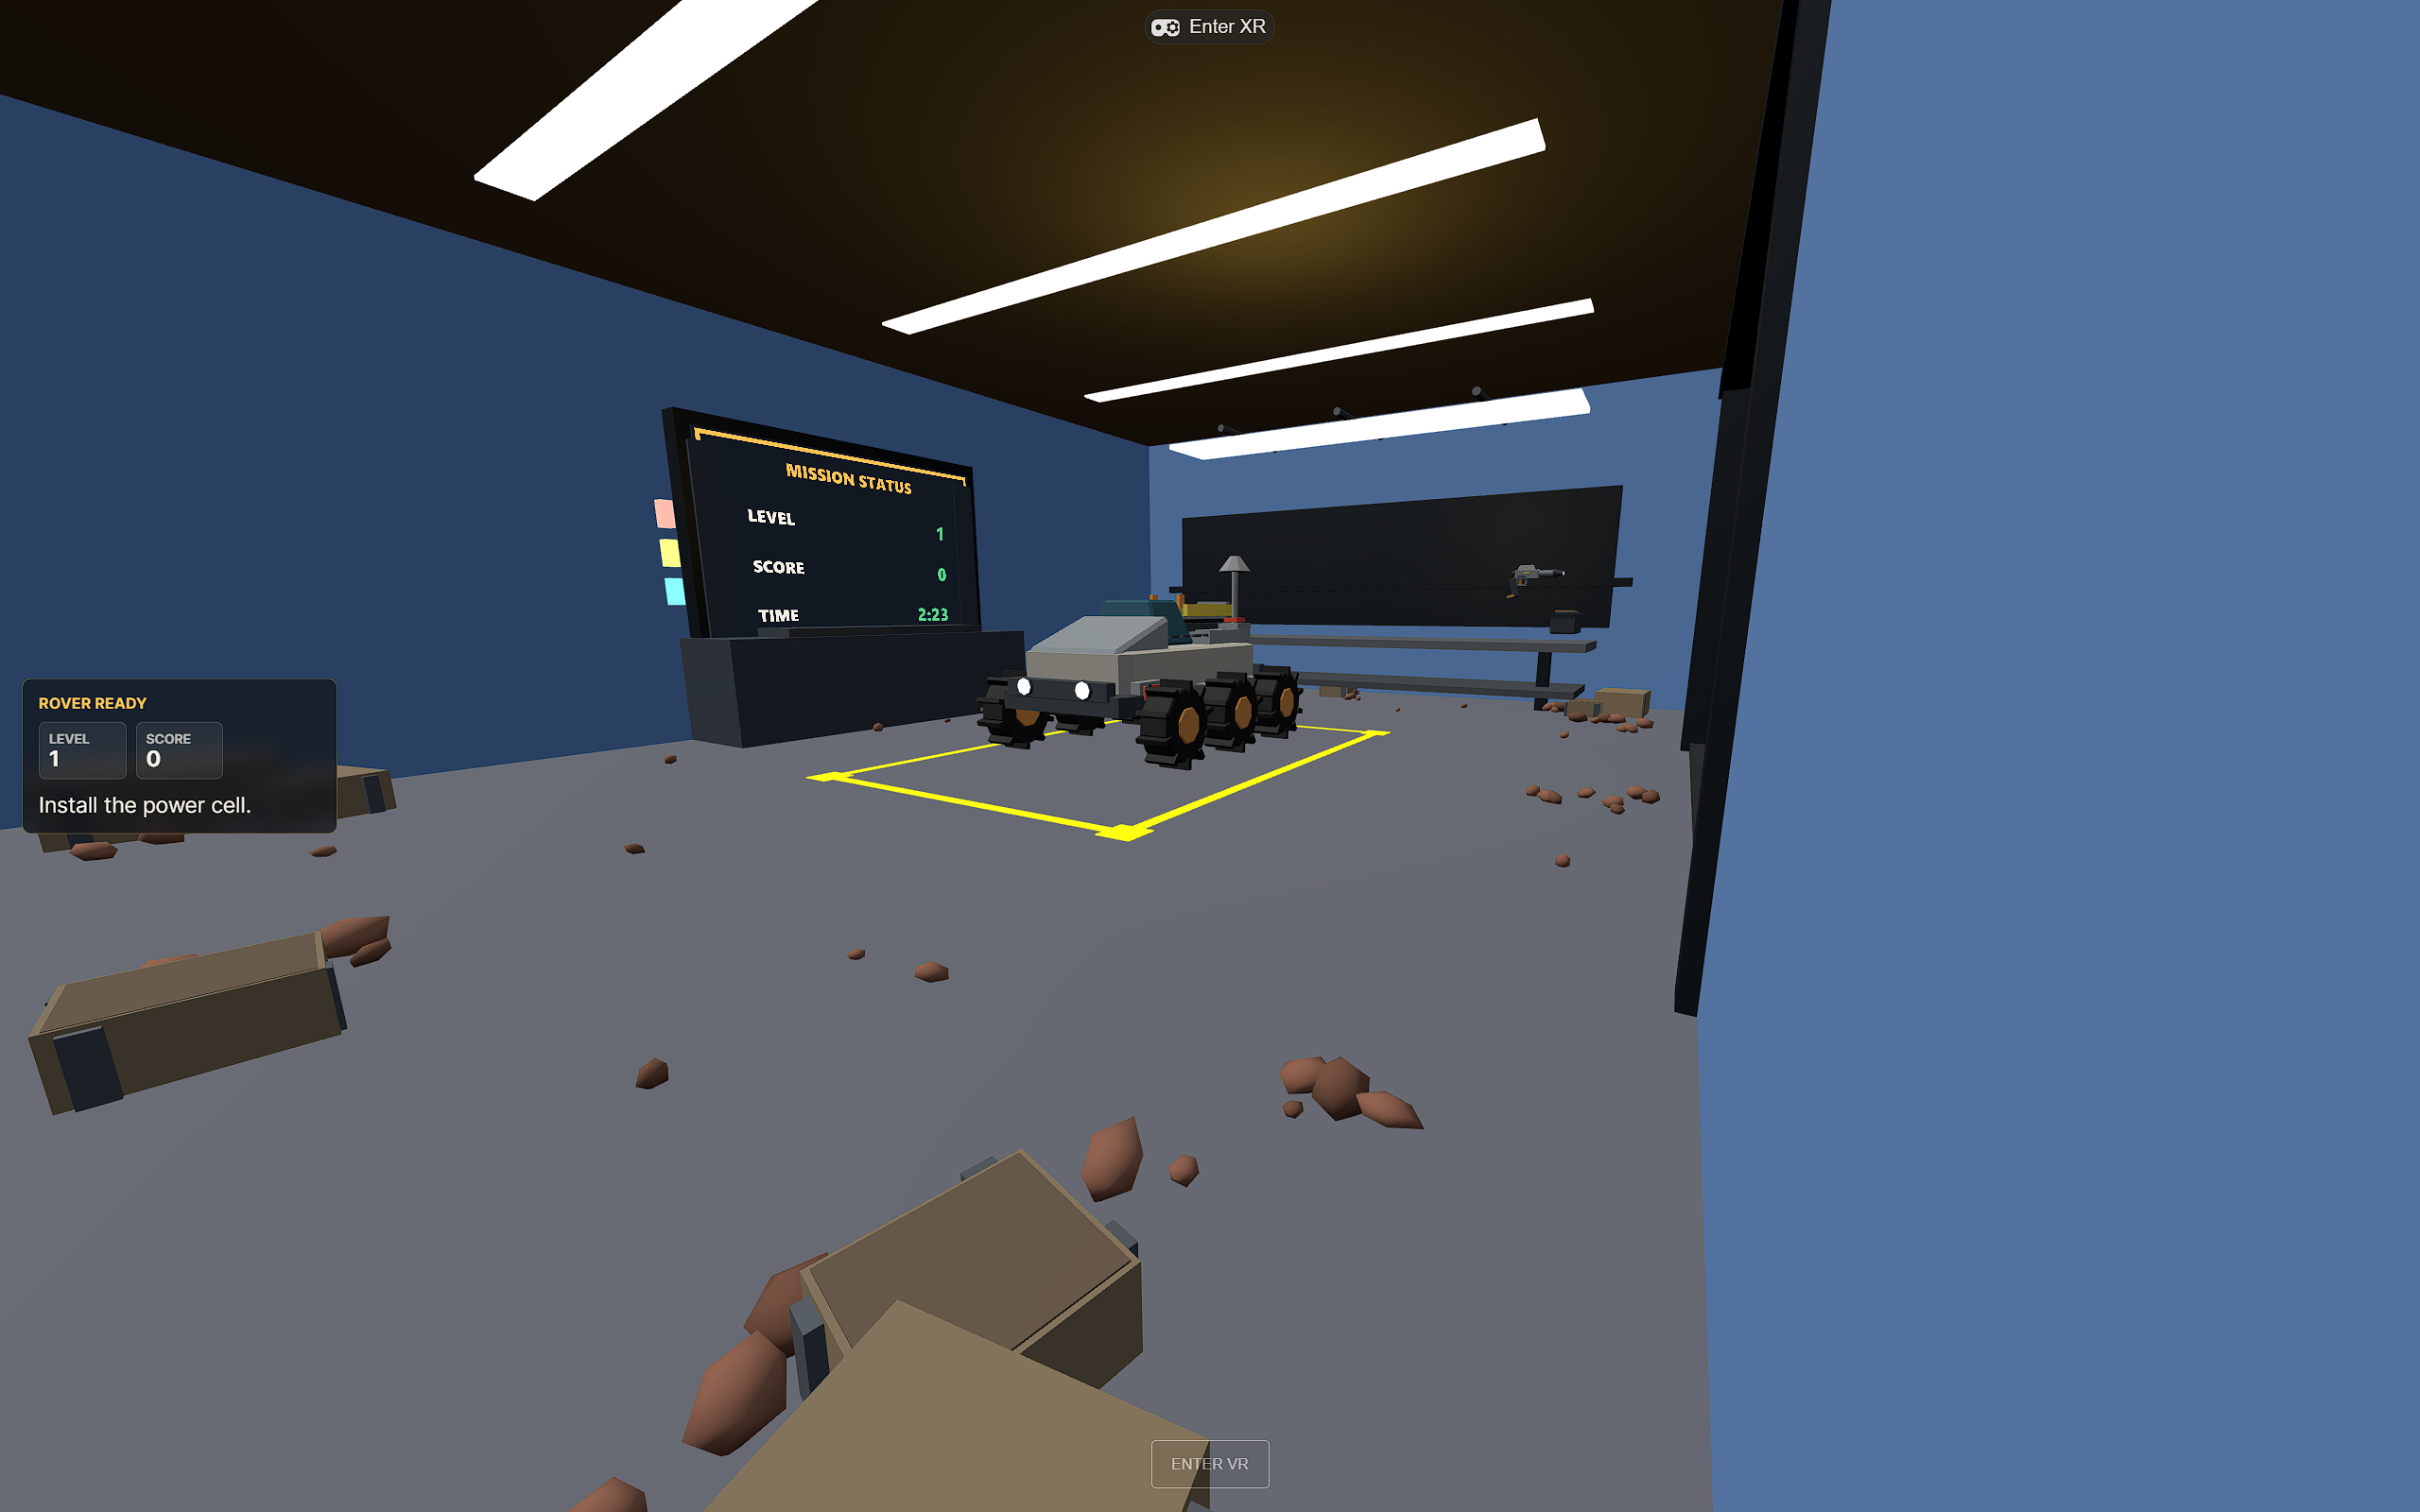
\includegraphics[width=0.32\textwidth]{setup.png}
	\hfill
	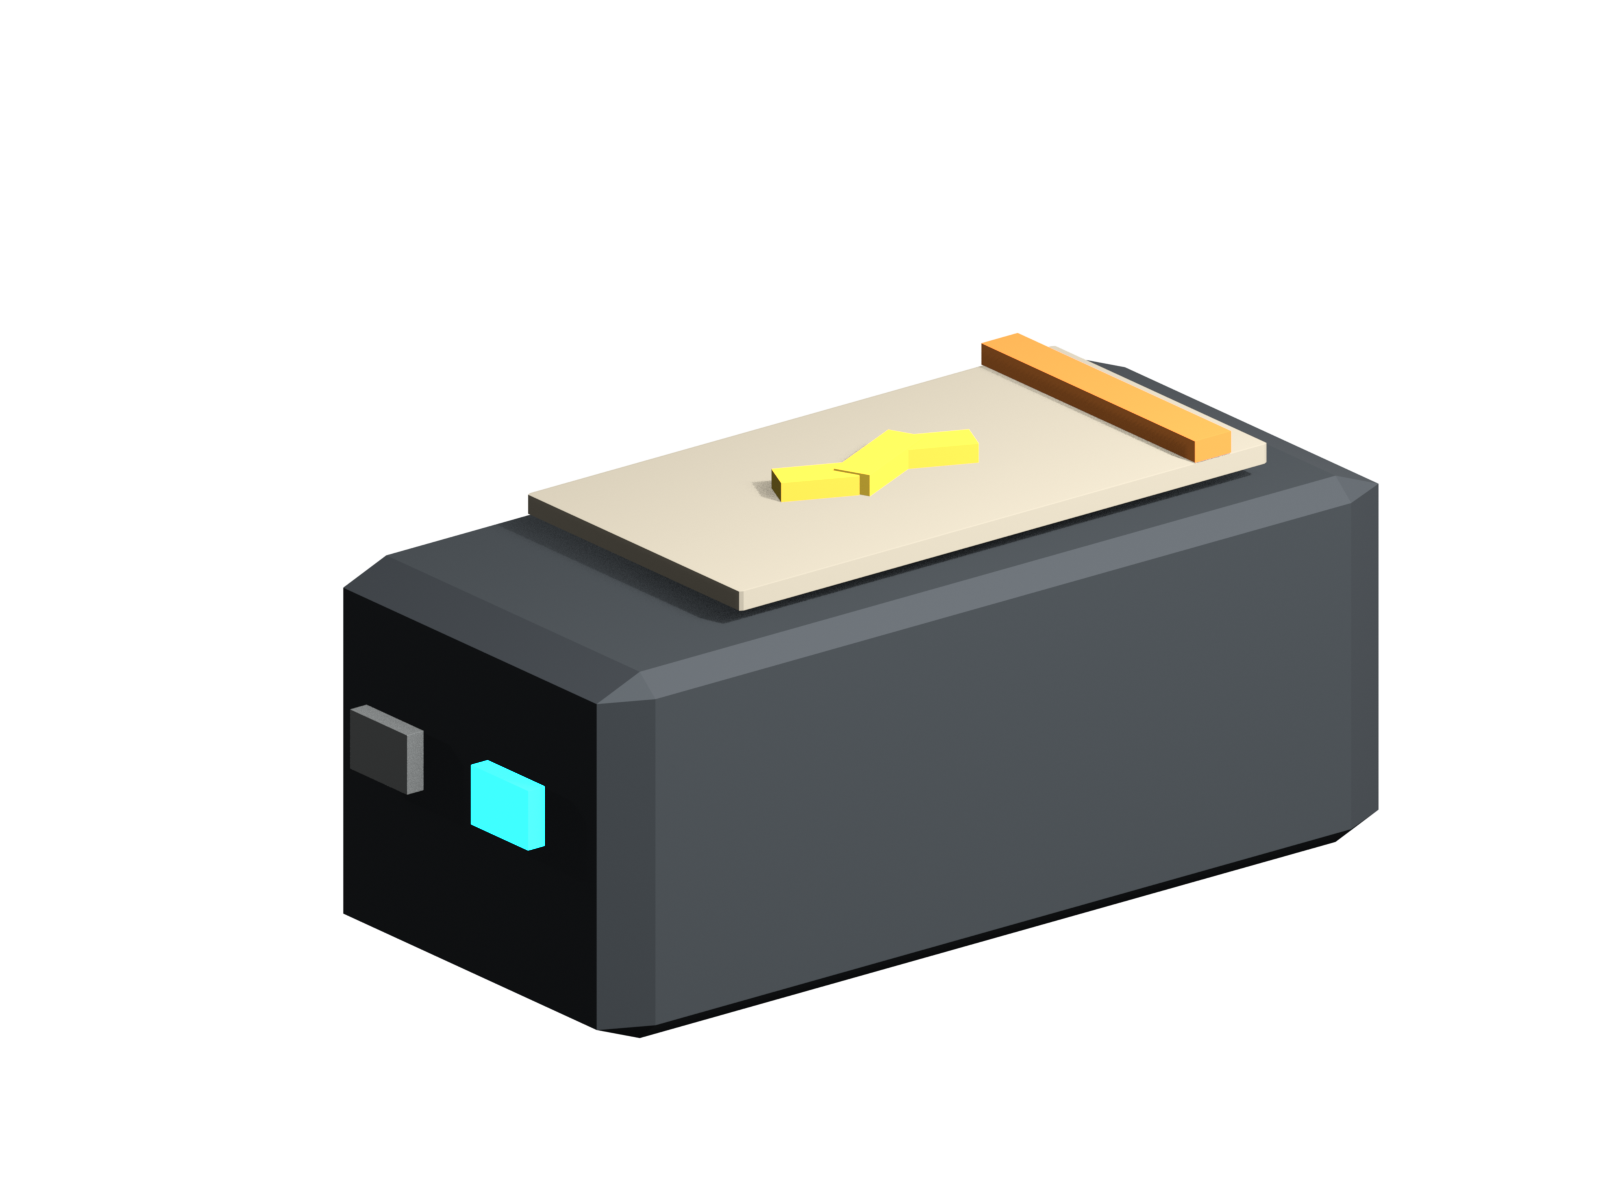
\includegraphics[width=0.32\textwidth]{power_module.png}
	\hfill
	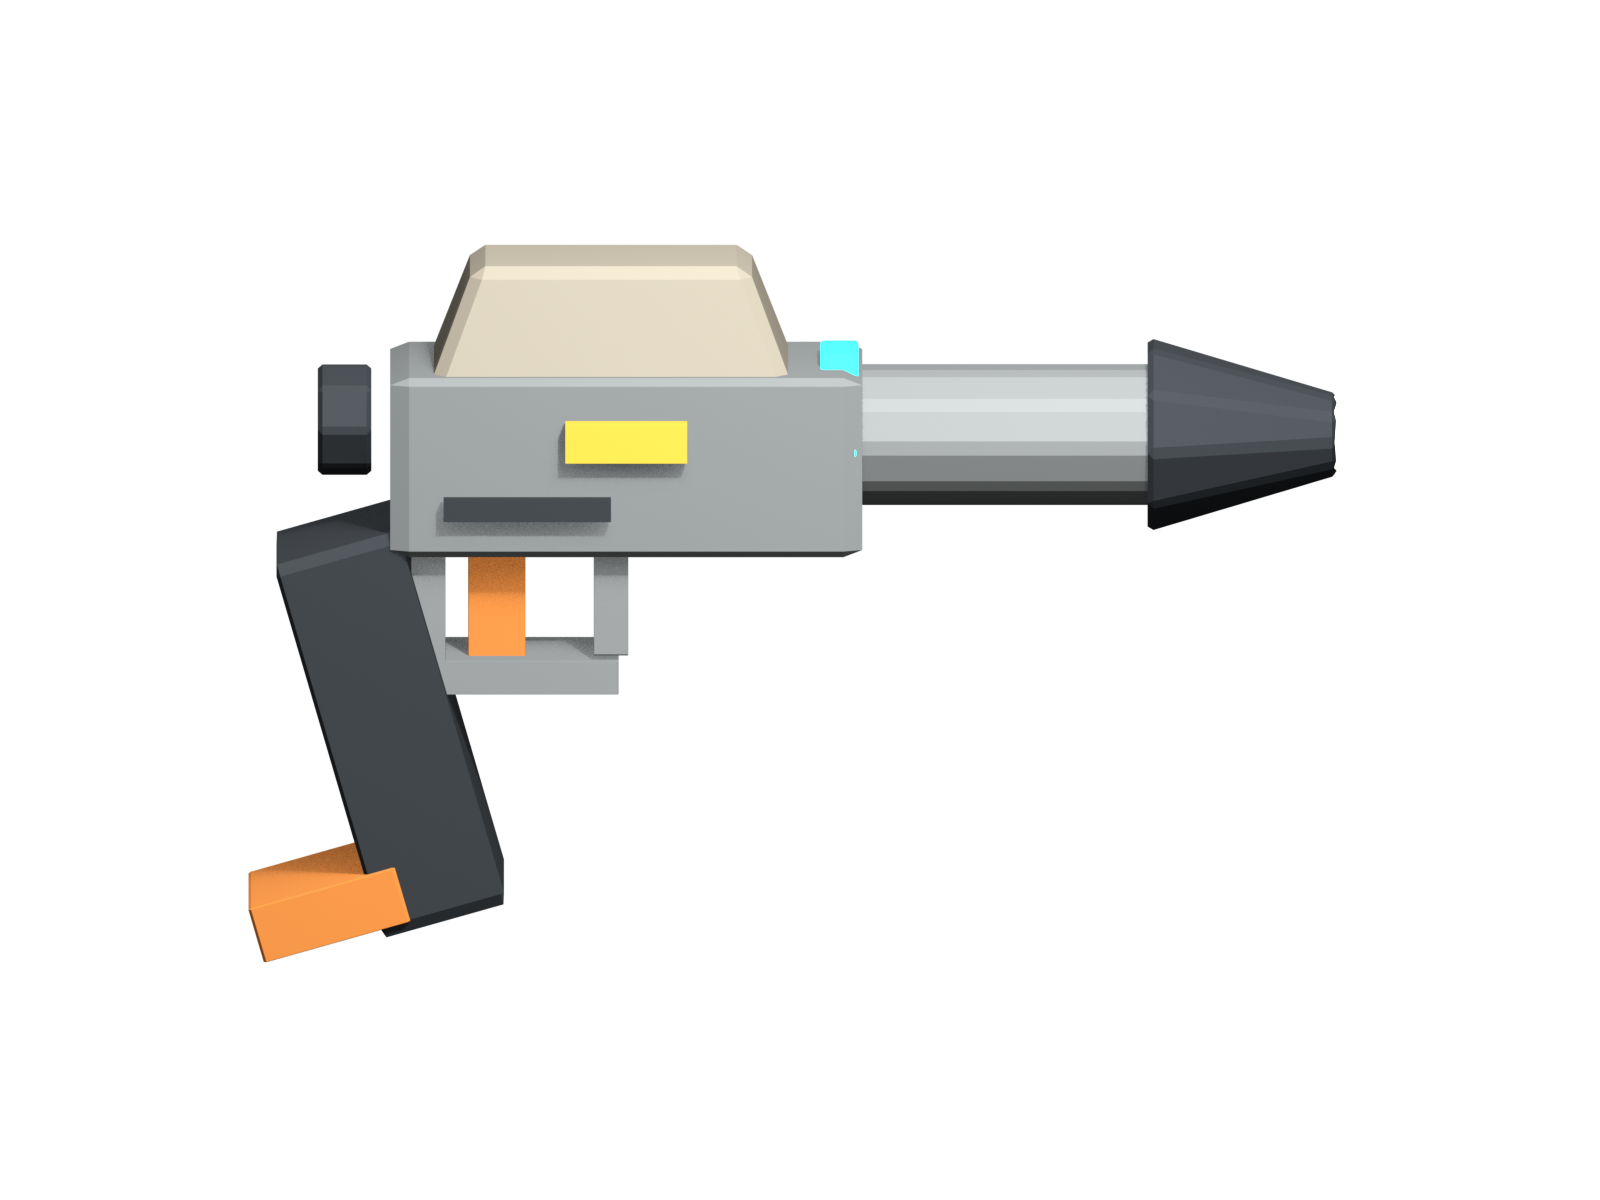
\includegraphics[width=0.32\textwidth]{repair_tool.png}
	\caption{Final demo visuals. Left: the rover parked inside the repair bay.
		Center: the custom power-cell module. Right: the custom handheld repair tool.}\label{fig:demo-visuals}
\end{figure*}

\section{Features Table}

Table~\ref{tab:features} summarizes how the project meets the base and advanced
feature requirements. The base requirements are separate from the advanced
feature count.

\begin{table*}[t]
	\caption{Requirement Coverage}\label{tab:features}
	\centering
	\footnotesize
	\begin{tabular}{llll}
		\toprule
		\textbf{Req.}      & \textbf{Type} & \textbf{Coverage}             & \textbf{Section} \\
		\midrule
		Original theme     & Base          & Compact rover repair bay      & Overview         \\
		Custom 3D assets   & Base          & Blender-made GLB models       & Overview, assets \\
		Core interactions  & Base          & Power, repair, parts, buttons & Scene            \\
		Physics            & Category A    & Cannon-ES objects and proxies & Challenges       \\
		Object types/modes & Category A    & Buttons, tools, parts, rovers & Scene            \\
		Blender generation & Supporting    & Python-generated assets       & Execution        \\
		\bottomrule
	\end{tabular}
\end{table*}

\section{Challenges and Solutions}

The largest challenge was keeping the Blender asset files and the browser
runtime aligned. A model can look correct in Blender while still having a snap
point, collision box, or interaction distance that feels wrong in WebXR\@. We
addressed this by giving important model nodes stable names, such as rover snap
targets and repair-tool use points, then looking them up by name in the
JavaScript runtime.

Physics stability was another challenge. Loose parts need to feel physical, but
VR interactions become frustrating if objects bounce away, fall through the
table, or collide with overly detailed visual geometry. The solution was to use
simple Cannon-ES proxy shapes for the objects and surfaces that matter to the
gameplay, while keeping the more detailed GLB meshes visual.

Scope control also mattered. The original idea could have expanded into a larger
Mars facility, but that would have reduced the time available for interaction
polish. The final build keeps the player inside one bay and increases challenge
through more repair targets, more missing parts, and the complex rover rather
than through new rooms.

\section{Discussion and Future Work}

The strongest part of the project is the clarity of the interaction loop. The
player can read the bay layout quickly: the rover stops in the marked work zone,
the tools are near the table, and the buttons control the rover flow. The snap
targets help the power-cell and missing-part interactions stay usable without
removing the feeling of physical placement.

The main limitation is feedback polish. The demo communicates state through the
HUD, glowing targets, object snapping, and button states, but sound effects,
stronger haptics, and more animated tool feedback would make the repair process
feel more complete. Headset testing could also be expanded beyond emulator and
desktop workflows.

With more time, we would add audio cues, clearer diagnostic-screen animations,
more varied repair jobs, and better end-of-level feedback when the rover leaves
the bay. We would keep those additions within the same garage-bay structure so
the project remains focused.

\section{Individual Contributions}

Table~\ref{tab:contributions} lists component ownership. The percentages are
approximate and describe the lead responsibility for each area.

\begin{table}[t]
	\caption{Individual Contribution Summary}\label{tab:contributions}
	\centering
	\footnotesize
	\begin{tabular}{lll}
		\toprule
		\textbf{Component}      & \textbf{Lead}   & \textbf{Approx. Share} \\
		\midrule
		Asset visual direction  & Chirag Baviskar & 60\% / 40\%            \\
		Asset export/package    & Chirag Baviskar & 70\% / 30\%            \\
		Three.js/WebXR runtime  & Dhrumil Patel   & 30\% / 70\%            \\
		Input handling          & Dhrumil Patel   & 30\% / 70\%            \\
		Physics and collisions  & Dhrumil Patel   & 30\% / 70\%            \\
		Game flow and HUD       & Dhrumil Patel   & 35\% / 65\%            \\
		Final docs/presentation & Chirag Baviskar & 60\% / 40\%            \\
		\bottomrule
	\end{tabular}
\end{table}

\section{Asset Credits}

The visible garage bay, rover models, power-cell module, repair tool, and Mars
exterior assets were made for this project using Blender and the Blender Python
scripts included in the source materials. The submitted source includes the
original \path{.blend} files, exported \path{.glb} runtime models, and generation
scripts.

The runtime uses Three.js for rendering and WebXR support, Cannon-ES for
physics, and browser WebXR APIs. These are external software libraries and APIs,
not third-party scene assets. No third-party 3D models, 360-degree media,
Gaussian splats, or external texture packs are used in the final visible scene.

\section{Code and Execution Instructions}

The runnable project is in the \path{final} folder. It must be served through a
local web server because it uses JavaScript modules, CDN imports, and GLB asset
loading. Do not open \path{index.html} directly from the file system.

From the \path{final} folder, run one of the included scripts:

\begin{verbatim}
.\run-demo.ps1
run-demo.bat
./run-demo.sh
\end{verbatim}

Each script serves the project at:

\begin{verbatim}
http://localhost:5173/
\end{verbatim}

The server can also be started manually from the \path{final} folder:

\begin{verbatim}
python -m http.server 5173
\end{verbatim}

Then open \url{http://localhost:5173/} in a Chromium-based browser. Desktop
testing uses \texttt{W}, \texttt{A}, \texttt{S}, and \texttt{D} for movement,
arrow keys for turning, and mouse drag for grabbing. VR testing uses WebXR
controller movement and trigger/select for grabbing. The WebXR Emulator browser
extension can be used when a headset is not available.

The source materials include \path{final/index.html}, all JavaScript under
\path{final/src}, runtime GLB files under \path{final/src/assets/models},
Blender source files under \path{final/src/assets/blend}, and Blender generation
scripts under \path{final/scripts/blender}. The packaged asset/source bundle is
\path{final/dist/rover_ready_assets.zip}.

\nocite{three,webxr,cannon,blender}
\bibliographystyle{IEEEtran}
\bibliography{refs}

\end{document}
